
\documentclass{lxaiproposal}
  
  
%   \usepackage[english,french]{babel}   % "babel.sty" + "french.sty"
\usepackage[english]{babel}   % "babel.sty" + "french.sty"
   
% \usepackage[english,francais]{babel} % "babel.sty"
% \usepackage{french}                  % "french.sty"
\usepackage{times}			% ajout times le 30 mai 2003
 
\usepackage{epsfig}
\usepackage{graphicx}
\usepackage{amsmath}
\usepackage{amssymb}
\usepackage{booktabs}
\usepackage{multirow}
\usepackage{pifont}
\usepackage{caption}
\usepackage{subcaption}
\usepackage{kotex}
\usepackage{hyperref}

\usepackage{array}
\usepackage{color}
\usepackage{colortbl}

\usepackage{pifont}
\usepackage{amssymb}
\usepackage{latexsym}

\usepackage{booktabs}

%% --------------------------------------------------------------
%% FONTS CODING ?
% \usepackage[OT1]{fontenc} % Old fonts
% \usepackage[T1]{fontenc}  % New fonts (preferred)
%% ==============================================================

\title{Open-Source Software Practice Final Project - Proposal Phase}

\author{\coord{Donghun Jung, }{2020312141}{1} \\
        \coord{Jinhwa Hong, }{2017310820}{2} \\
        \coord{hyeonjeong Ko, }{2020315791}{3} \\
}

\address{
    \affil{1}{Sungkyunkwan University, Department of Physics, }{\texttt{atompioneer@g.skku.edu}}
    \affil{2}{Sungkyunkwan University, Systems Management Engineering, }{\texttt{bout123456@naver.com}}
    \affil{3}{Sungkyunkwan University, Department of software, }{\texttt{toyu7870@naver.com}}
}

%% If all authors have the same address %%%%%%%%%%%%%%%%%%%%%%%%%%%%%%%%%%%%%%%
%                                                                             %
%   \auteur{\coord{Michel}{Dupont}{},                                         %
%           \coord{Marcel}{Dupond}{},                                         %
%           \coord{Michelle}{Durand}{},                                       %
%           \coord{Marcelle}{Durand}{}}                                       %
%                                                                             %
%   \adress{\affil{}{Laboratoire Traitement des Signaux et des Images \\      %
%     1 rue de la Science, BP 00000, 99999 Nouvelleville Cedex 00, France}}   %
%                                                                             %
%                                                                             %
%%%%%%%%%%%%%%%%%%%%%%%%%%%%%%%%%%%%%%%%%%%%%%%%%%%%%%%%%%%%%%%%%%%%%%%%%%%%%%%

% \englishabstract{}

\begin{document}
\maketitle
%
\section{Application type}
\vspace*{-3mm}
웹페이지 기반

\section{Theme}
\vspace*{-3mm}
주제 : 성균튜터링 신청 사이트

해당과목에서 A이상 학점을 받은 튜터와 학습에 도움을 받고자 하는 튜티들이 그룹학습을 할 수 있도록 매칭하고 지원하는 프로그램이다.
매학기 약 500여명이, 100여 개의 팀으로 참여하여, 튜터를 중심으로 스터디를 이끌어간다.
많은 학생들이 참여하는 활동임에도 불구하고 신청 과정은 꽤 불친절하다. 

\begin{figure}[h]
    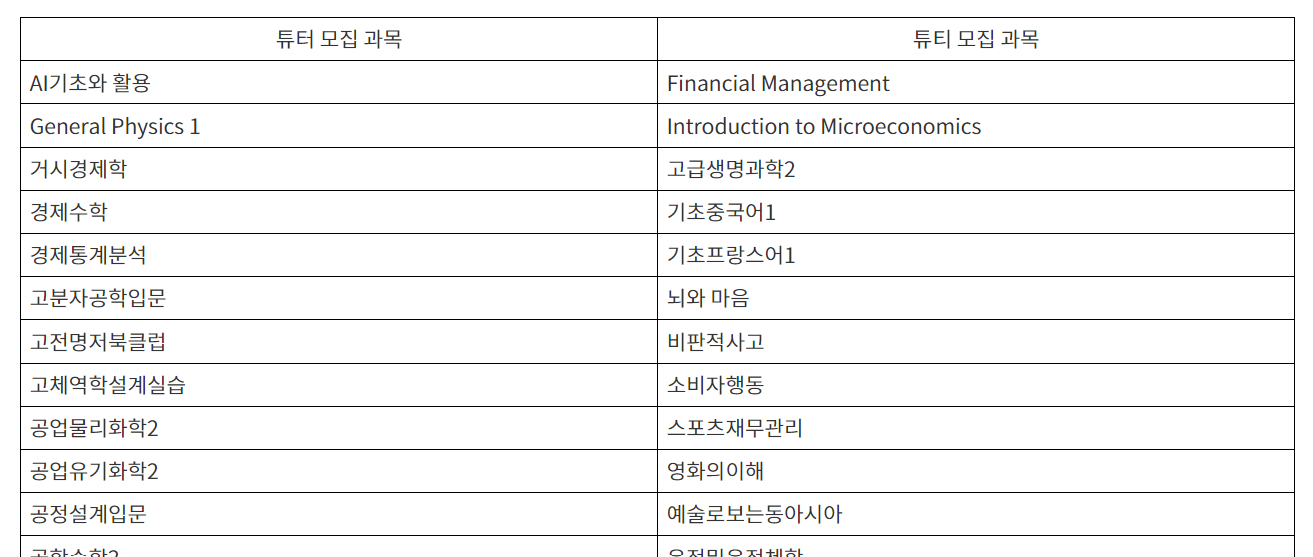
\includegraphics[width = 0.45\textwidth]{Fig1.png}
    \caption{성균튜터링 신청 과목 현황 예시}
\end{figure}
첫째로, 어떤 과목이 개설되어 있는지 확인하기 어렵다.
그림 1에서 확인할 수 있는 것처럼 교육개발센터에서 신청 마감 약 이틀전부터 모집 과목을 업로드해준다. 튜터와 튜티 모두 어떤 과목이 필요하고 개설되는지 확인하기 어렵다. 

둘째로, 튜터링을 신청하면서도 성사여부를 확신할 수 없다. 개설여부를 즉시 확인하기 어렵기도 하고, 모집마감 여부 역시 불투명하기 때문이다. 이는 튜터링 신청을 주저하는 원인 중 하나이기도 하다.

셋째로, 튜터가 튜터링을 신청할 때에 제공하는 많은 정보를 제공하는 것에 반해, 튜티는 랜덤으로 튜터를 배정받는다. 
튜터로 튜터링을 신청할 때, 본인의 성적, 수강한 과목의 담당교수, 커리큘럼, 지원동기 등을 입력하나 튜티가 신청할 때에 관련된 정보를 전혀 얻을 수 없다.
교육개발센터에서는 담당교수만을 중심으로 학생을 배정하고 있다. 해당 정보들을 모두 공개하여 튜티가 튜터를 선택하게 할 수 있는 것이 바람직하다.

마지막으로, 공지는 학교 홈페이지, 신청은 구글폼, 결과 확인은 교육개발센터 네이버 카페에서 이루어지는 번거로움이 있다.

이런 이유로, 성균튜터링 신청 사이트를 이번 프로젝트 주제로 선정하여 성균튜터링 신청 사이트를 제작하고자 한다.

\section{Sketch}
\vspace*{-3mm}
학교 수강신청 사이트와 유사할 것으로 예상.(그림 첨부 요망)

\section{Features}
\vspace*{-3mm}

현재 구상중인 기능은 아래와 같다.
\subsection{로그인 기능}
학번(id), 이름(혹은 비밀번호)를 통해 로그인

\subsection{튜터링 과목 등록}
튜터가 튜터링할 과목을 선택하고 튜터링 신청.
입력해야 받아야 할 정보는 다음과 같음.
\begin{enumerate}
    \item 취득 성적(A+/A)
    \item 과목명
    \item 수강한 교수명
    \item 튜터링 계획(Syllabus)
    \item 지원 동기
    \item 그룹 지원 여부 및 튜티 학번
    \item 가능한 시간 등등
\end{enumerate}

\subsection{튜터링 수강 신청}
튜티가 튜터가 등록한 정보를 확인하고, 신청.
튜티에게 보여져야하는 정보는 다음과 같음.
\begin{enumerate}
    \item 과목명, 튜터명, 시간 등 기본적인 정보
    \item 자세히 보기와 같은 버튼을 통해 열람 가능한 취득성적, 교수명, 튜터링 계획 등 자세한 정보
    \item 신청 현황 (n/5와 같이 표기)
\end{enumerate}

\section{Usage scenario}
\vspace*{-3mm}
\subsection{회원가입}
학번과 이름(혹은 pw)를 입력받아 회원가입.
if 존재하는 학번 -> 실패
else 유저목록에 새로 등록

\subsection{로그인}
학번과 이름(혹은 pw)를 입력받고 일치하면 튜터링 신청 화면으로 전환.
https request를 통해 입력 받은 정보를 보내고 일치여부를 수신 받아야 함. 일치하지 않을 시 알림 띄우기.

\subsection{튜터 과목 등록}
과목 등록 시, 다음 정보를 입력 받아야 함.
\begin{enumerate}
    \item 취득 성적(A+/A)
    \item 과목명
    \item 수강한 교수명
    \item 튜터링 계획(Syllabus)
    \item 지원 동기
    \item 그룹 지원 여부 및 튜티 학번
    \item 가능한 시간 등등
\end{enumerate}
취득성적이 A 미만인 경우, 과목 등록이 불가능.
과목명은 학교 GLS에서 크롤링해온 과목 목록에 존재해야 함.
튜티 학번은 유저 목록에 존재해야 함.

\subsection{튜티 수강 신청}
과목 목록에 과목명, 튜터명, 튜터링 시간 등 기본적인 정보 확인 가능.
신청 버튼과 자세히 보기 버튼을 누름으로써 인터페이스와 상호작용함.
신청하기 버튼을 누르면 해당과목에 신청한다는 request를 서버에 보내고 가능여부를 서버로부터 수신 받음.
if 신청 인원 초과 or 이미 신청한 튜터링 -> 불가능 메세지 출력
else 수락 메세지 출력 및 (신청 인원)++
자세히 보기 버튼을 누르면 취득성적, 교수명, 튜터링 계획 등 자세한 정보 확인

\section{Task assignment}
\vspace*{-3mm}

위 기능을 구현하기 위해 다음 작업이 필요할 것으로 예상된다.
\subsection{AWS 서버 구축}
학교에 개설된 과목 목록, 유저 목록, 튜터링 과목 목록을 저장하고 http request를 송수신할 서버 구축

\subsection{MVC, MVP, MVVP 모델}
AWS 서버로부터 튜터링 과목 목록을 수신받고 화면에 출력할 cell을 만들기 위해 필요.

\subsection{Http request}
AWS 서버와 정보를 주고받는 수단.

\subsection{Webpage design with HTML}


\subsection{JS code}
http request 송수신과 관련된 코드.

\subsection{crawling}
학교 GLS에 존재하는 과목을 끌와 AWS 서버에 저장

% \bibliographystyle{ieee_fullname}
% \bibliography{references}

%\begin{thebibliography}{99}
%\end{thebibliography}

\end{document}
